\chapter{\label{ch:6-discussion}Discussion}
\minitoc{}

\section{Overview}

% So far, this thesis has:

% \begin{itemize}
%   \item established relapse as clinically significant VL outcome, both for individual patients and regional elimination efforts (Chapter \ref{ch:2-background}),
%   \item demonstrated that, despite its importance, no models predicting relapse exist, identifying a clear and important gap in the literature (Chapter \ref{ch:3-sys-review}), and
%   \item developed and internally validated four relapse prediction models for patients in the ISC and East Africa (Chapters \ref{ch:4-isc-model-methodology}--\ref{ch:6-ea-model-results}).
% \end{itemize}

Drawing on prospectively collected data from 6,650 participants across 19 prospective studies, the models presented in this thesis constitute the first attempt to predict visceral leishmaniasis relapse at the individual patient level.

Despite considerable heterogeneity across the contributed studies and substantial missing data \textemdash\ necessitating the use of novel statistical approaches \textemdash\ several important predictors of relapse were identified. Fever duration and baseline parasite grade showed effects shared across both East Africa and the ISC, supporting their role as core prognostic factors. Other predictors demonstrated region-specific effects: the association between anaemia and relapse differed in direction between regions, WBC count and malnutrition were predictive only in East Africa, and age only in the ISC. Models incorporating parasite grade achieved superior discrimination, especially in East Africa. However, in the ISC, excluding parasite grade still allowed for meaningful model performance.

\subsection{Chapter Structure}

This final chapter provides a structured reflection on the presented models. Insights from preceding chapters are drawn upon to provide context and assess the implications of the presented prediction models.

First, the mechanistic plausibility of the identified predictor-relapse relationships is explored \textemdash\ `\textit{what do the models teach us about the nature of VL relapse?}'. Specifically, a causal framework is developed that links the model predictors with VL relapse. This approach supports user confidence in the models, and provides a tool for discovery that can generate new hypotheses and insights into the underlying disease process.

Second, key strengths and limitations are explored relating to the underlying data, study design, and assumptions made during the modelling process. Issues related to model performance, interpretability, and generalisability are discussed. The potential impact of the developed models on clinical practice is considered.

Third, directions for future research are explored. These include how data-driven approaches can be leveraged to shine new light onto both the nature and determinants of VL relapse, and how such efforts can be translated into policy.

\section{Plausibility of Relapse Predictors}

It merits emphasis that the identified relapse-predictor relationships, as illustrated in Figures~\ref{fig:isc_var_forest_combined} and \ref{fig:ea_var_forest_combined}, simply reflect statistical associations arising under the stated modelling assumptions. Predictive accuracy does not imply biological plausibility. However, offering a mechanistic framework can add substantial value. Specifically:

\begin{description}
  \item{\textbf{User confidence}}. Biological plausibility improves the face validity of the models, increasing user trust in their predictions.
  \item{\textbf{Model applicability}}. By clarifying which associations are likely to remain stable, a mechanistic understanding informs the extent to which a model can be applied across different populations, settings, and time periods.
  \item{\textbf{Tool for discovery}}. Model findings, when interpreted through a mechanistic lens, can generate hypotheses and contribute to a broader understanding of the underlying disease process.
\end{description}

Given these benefits, this section aims to build on the disease pathophysiology set out in Chapter~\ref{ch:1-background}, and provide additional context to the model findings.

\subsection{Parasite Dynamics}

Supporting a more mechanistic interpretation, Figure~\ref{fig:natural-history} schematically illustrates the temporal dynamics of parasite load before, during, and after treatment. The figure situates relapse within the broader natural history of infection and treatment response, contextualised as four interconnected stages: asymptomatic stage $\rightarrow$ symptomatic stage $\rightarrow$ treatment stage $\rightarrow$ post-treatment stage.

In Chapter~\ref{ch:1-background}, studies identifying factors predictive of relapse were systematically reviewed and presented in Table~\ref{tab:relapse-rf}. By considering the natural history of disease, and how relapse predictors relate to the underlying pathophysiological processes occurring at each stage, we can better understand the mechanistic plausibility of the observed predictor-relapse relationships.

\newgeometry{left=1.5cm, bottom=2.5cm, right=2cm, top=3cm}
\begin{landscape}
  \begin{figure}[tb]
    \centering
    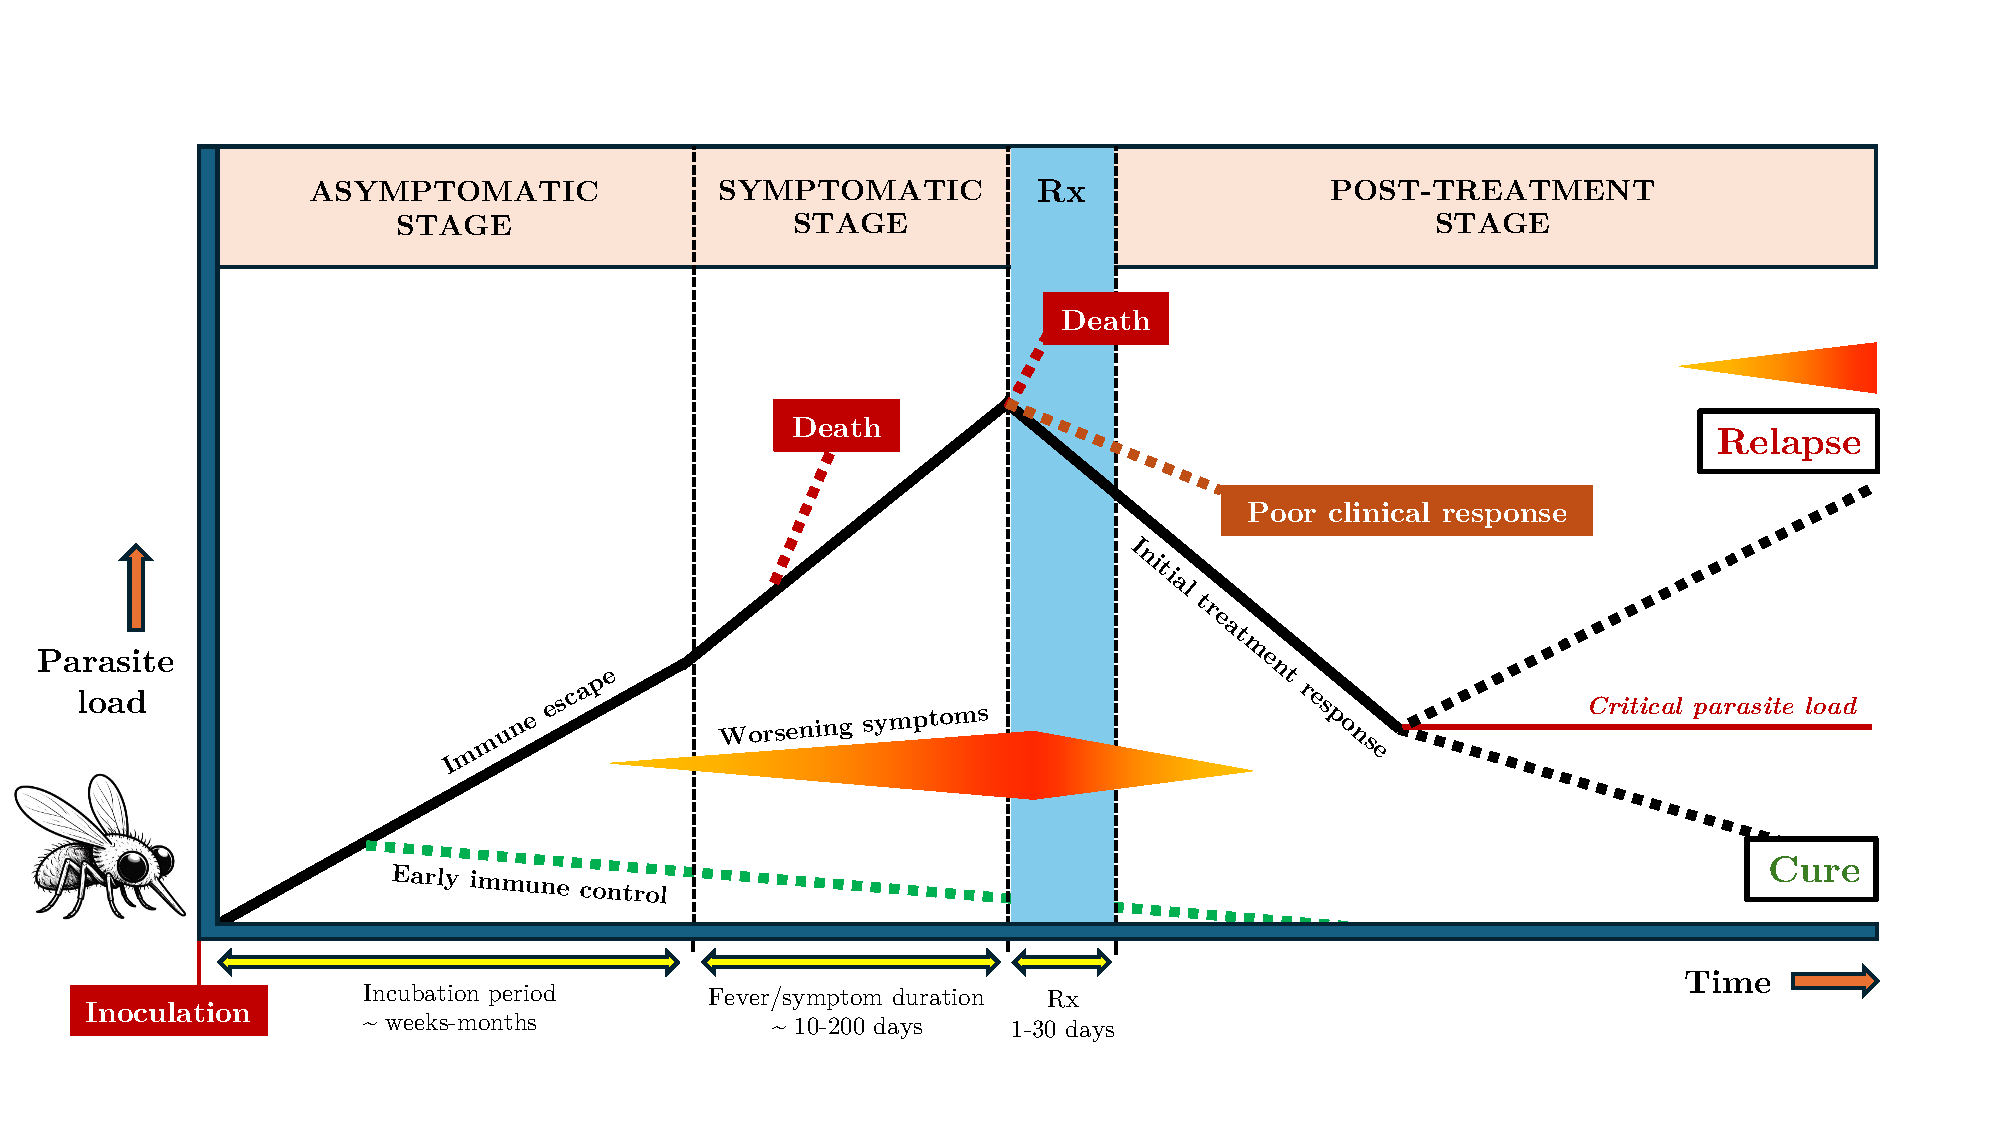
\includegraphics[width=\linewidth, trim = {0.2cm 1.2cm 2cm 2.4cm}, clip]{figures/ch6/natural-history.pdf}
    \caption{Schematic of the evolution of parasite load during VL infection. Events occurring during the post-treatment stage are critical in determining subsequent relapse. It is hypothesised that for each individual patient, a post-treatment `critical parasite load' defines the threshold below which the host immune system controls parasite replication resulting in lasting cure. The threshold itself depends on (i) the pre-treatment parasite load, (ii) the degree of parasite depletion by treatment, (iii) host immunity, and (iv) the intrinsic parasite virulence. Rx: treatment, PKDL: post-kala-azar dermal leishmaniasis.}
    \label{fig:natural-history}
  \end{figure}
\end{landscape}
\restoregeometry

\subsubsection{From Asymptomatic Infection to Symptomatic Disease}

In endemic areas, cross-sectional surveys demonstrate that approximately 10--30\% of individuals harbour asymptomatic infection\cite{mannan2021}. However, only a minority of these individuals progress to symptomatic disease, underscoring that clinical illness represents the exception rather than the norm in infected populations\cite{hasker2014}. Primary disease progression reflects a complex interplay of host genetic susceptibility, immune competence, and parasite-related factors, although these relationships remain poorly understood\cite{kaye2011}.

Relapse shares a key conceptual feature with primary disease progression \textemdash\ namely, a failure to control parasite expansion and the transition from an asymptomatic to symptomatic state. Therefore, studies examining determinants of primary disease progression can also provide insights into the mechanisms underlying relapse. High-quality prospective incidence studies are particularly informative in this regard, and provide important context for upcoming discussions\cite{picado2010,hasker2014,bern2007}.

\subsubsection{Progression of Symptomatic Disease}

As symptoms evolve, immune control is progressively undermined by parasite immune evasion, facilitating intracellular persistence and dissemination within the mononuclear phagocytic system. Host immune responses become increasingly skewed toward an immunoregulatory profile associated with dysfunctional cell-mediated immunity. This shift drives a vicious cycle of immunosuppression, heightened susceptibility to co-infections, and progressive end-organ damage\cite{kaye2011,costa2023}.

Historical descriptions from the pre-treatment era reveal marked variability in the natural history of disease. Nineteenth-century outbreaks in Assam and Bengal were characterized by devastating epidemic cycles, with rapid disease progression and mortality exceeding 90--95\%\cite{sengupta1947,gibson1983}. In contrast, in settings with endemic disease, a more chronic, relapsing-remitting course is described that could persist for years\cite{sengupta1947}.

Understanding how clinical and laboratory factors evolve during symptomatic disease can help explain a number of relapse predictors, including fever duration, splenomegaly, anaemia, WBC count, and parasite grade. Drawing on literature that describes the natural progression and inter-relatedness of these factors can offer a framework for interpreting their mechanistic links to relapse.

\subsubsection{Treatment Stage}

Treatment decisions \textemdash\ including the choice of drug, dose, and duration \textemdash\ are central to determining whether, and to what extent, a patient improves clinically and biochemically. As discussed in Chapter~\ref{ch:1-background}, with effective treatment, quantitative molecular markers of blood parasite load decrease from the order of \textasciitilde 10$^3$--10$^5$ parasites/ml at treatment initiation to \textasciitilde 10$^0$--10$^1$ parasites/ml by day 28, although with substantial variation between treatment regimens and individuals. Symptomatic improvement and subsequent relapse have been shown to be correlated with end-of-treatment parasite burden\cite{sudarshan2011,verrest2021,verrest2024,takele2023}.

% this could move to the introduction
\subsubsection{\textit{Do Predictors of Initial Treatment Failure Also Predict Relapse?}}

Relapse, by definition, is contingent on an initial clinical, and often parasitological response to treatment, and reflects failure to achieve sustained parasite clearance. This raises the question of whether risk factors for initial treatment failure are also risk factors for relapse. If so, predictors identified in studies of treatment failure could be extrapolated to better understand relapse risk. However, answering this question requires careful consideration of both how initial treatment failure is defined and the underlying pathophysiological processes it captures.

In analyses based on routine care data, where restrictive inclusion criteria are not applied, the most common cause of initial treatment failure is often death during treatment. This is illustrated by Yeshaw et al.\ (2020)\cite{yeshawIncidenceMortalityIts2020}, who reported that among 568 adult patients admitted to the University of Gondar Hospital, Ethiopia, between 2013 and 2017, 65 (11.1\%) patients died during treatment, whereas only 9 (1.5\%) were classified as treatment failures due to poor clinical response or persistence of parasites at the end of treatment. Notably, 60\% of deaths occurred within the first 10 days of treatment. Similarly, in Brazil, Maia-Elkhoury et al.\ (2019)\cite{maia-elkhoury2019} showed that among 1,589 visceral leishmaniasis deaths reported nationally between 2007 and 2014, the median time from notification to death was 9 days (IQR: 4--17 days). Comparable patterns have been reported in other settings\cite{kaminkClinicalSeverityScoring2017,werneckPrognosticFactorsDeath2003,alemu2023}.

In these contexts, early mortality \textemdash\ the most common cause of initial treatment failure \textemdash\ occurs due to advanced disease at presentation with severe organ dysfunction. Consequently, and as described in Chapter~\ref{ch:2-sys-review}, risk factors for mortality reflect the degree of organ dysfunction prior to treatment. These patients never reach a post-treatment state in which relapse can occur. Extrapolating predictors of initial treatment failure from these settings to relapse is therefore mechanistically inappropriate, given the distinct underlying pathophysiologies.

By contrast, in low-mortality settings without significant drug resistance, or in studies that exclude patients with severe disease, initial treatment failure is a rare event. When initial treatment failure occurs, it often reflects a positive test-of-cure, despite evidence of clinical improvement\cite{sundar2012,musa2023}. In this context, initial treatment failure better reflects inadequate parasite suppression, which is already established as an important predictor of relapse\cite{sudarshan2011,verrest2021,verrest2024}. Therefore, in such settings, observed treatment failure may function more as a surrogate marker of future relapse risk than as an indicator of true clinical non-response. However, depending on study outcome definitions, initial treatment failure may also include patients who discontinue treatment due to drug toxicity, or those who abandon therapy for non-biological reasons, further contributing to outcome heterogeneity.

On reflection, initial treatment failure is a heterogeneous construct that varies substantially across studies and settings, frequently encompassing multiple underlying processes, including death due to advanced disease, treatment discontinuation due to adverse events, and inadequate parasite suppression. The relative contribution of these components depends on the patient population, clinical setting, and study design. While initial treatment failure defined by parasitological non-response in low-mortality settings may serve as a proxy for relapse risk (inadequate parasite suppression), in high-mortality settings, or when treatment also captures discontinuation due to adverse events, extrapolating risk factors from initial treatment failure to relapse is likely misleading at best.

\subsubsection{Post-treatment Stage}

Expert consensus holds that VL treatment rarely results in sterile cure, as evidenced by animal models\cite{murray1996}, the persistence of serological markers following clinical cure\cite{gidwani2011}, the frequent detection of viable parasites at test-of-cure despite no subsequent relapse\cite{verrest2021}, case reports of disease reactivation many years after initial exposure\cite{eichenberger2017, postorino2011}, and the recent detection of quiescent parasites within bone marrow niches\cite{dirkx2024}. Instead, treatment is thought to suppress parasite burden to a level that allows for reconstitution of the host's cell-mediated immune response and subsequent parasite control\cite{murray1996, khalil2005}. In this context, relapse reflects a failure to achieve sustained parasite suppression, despite an initial treatment response. Events that occur following treatment are therefore critical in determining whether relapse occurs.

Verrest et al.\ (2024)\cite{verrest2024} hypothesise that post-treatment parasite dynamics are dependent on four key factors: (i) the pre-treatment parasite burden, (ii) the degree of parasite depletion by the treatment, (iii) the intrinsic parasite virulence, and, crucially, (iv) the host's immune system. It can be further hypothesised that, during the post-treatment stage, for each individual there exists a `critical parasite load' (Figure~\ref{fig:natural-history}). The threshold itself would be expected to vary between individuals, reflecting both differences in host immunity and in parasite virulence. For parasite loads below this threshold, the host immune system controls parasite replication resulting in lasting cure. For parasite loads above this threshold, parasite replication outpaces immune control, leading to relapse (Figure~\ref{fig:natural-history}).

\subsection{Causal Model for Relapse\label{sec:causal_model}}

Building on Verrest et al.'s hypothesis, a causal (mechanistic) model can be assembled. In this putative model, three key drivers of relapse, all shaped by events prior to and during treatment, determine whether relapse occurs: (i) post-treatment parasite grade, (ii) host immunity, and (iii) parasite fitness. Post-treatment parasite grade itself can be considered a direct consequence of both pre-treatment parasite grade and the treatment regimen. If presented as a directed acyclic graph (DAG), these drivers constitute the final common pathway (mediators) for relapse. In Figure~\ref{fig:dag}, text boxes (`nodes') represent relapse determinants, and lines (`vertices') indicate the direction of causality between nodes. For example, pre-treatment host immunity directly affects the initial rate of symptom progression.

Caution is advised, however, when interpreting such a model. As with DAGs for any disease process, they represent a broad approximation of true biological events and often fail to capture the nuanced dynamic interactions between outcome determinants as the disease evolves. Rarely do disease experts agree on the `correct' DAG\cite{daveysmith2016}. Limitations aside, the proposed DAG at least provides an explicit, albeit speculative, framework on the causes of relapse, motivating further debate and hypothesis generation.

\definecolor{green_dag}{RGB}{217,242,208}
\definecolor{pink_dag}{RGB}{242,207,238}
\definecolor{blue_dag}{RGB}{21,96,130}
\definecolor{orange_dag}{RGB}{255,192,0}

\begin{figure}[tb]
  \centering
  \includegraphics[width=\linewidth, trim = {5cm 5cm 7.5cm 1.1cm}, clip]{figures/ch6/dag.pdf}
  \caption{Directed acyclic graph (DAG) describing putative effectors of visceral leishmaniasis relapse. Factors are colour coded:\\ \colorbox{green_dag}{Factors measurable at the time of treatment initiation} \\ \colorbox{pink_dag}{Factors measurable at time of disease onset, or shortly thereafter} \\ \colorbox{blue_dag}{\textcolor{white}{Factors on the final common pathway to relapse}} \\ \colorbox{orange_dag}{Relapse}}
  \label{fig:dag}
\end{figure}

\subsection{Parasite Grade}

In both the ISC and East Africa, higher pre-treatment parasite grade was strongly associated with increased relapse risk. For each unit increase in parasite grade (i.e.\ from 1+ to 2+), the adjusted odds of relapse increased by 31\% in the ISC (aOR 1.31, 95\% CI 1.12--1.52) and 43\% in East Africa (aOR 1.43, 95\% CI 1.23--1.66).

This association is supported by evidence from diverse patient populations. Among 146 patients with VL/HIV co-infection in Ethiopia, of whom 44 (30\%) relapse, Abongomera et al.\ (2017) reported that a pre-treatment parasite grade of 6+ was strongly associated with relapse (HR 6.6, 95\% CI 2.6--16.6)\cite{abongomera2017a}. In 177 immunocompetent patients enrolled in East African DND\textit{i} trials (27 [15\%] relapse rate), Verrest et al.\ (2021) demonstrated that pre-treatment parasitaemia, measured by blood qPCR, was significantly lower in those who achieved definitive cure compared to those who relapsed (p = 0.03)\cite{verrest2021}. Similar findings were reported in India by Sudarshan et al.\ (2014)\cite{sudarshan2014}. Parasite load assessed by blood qPCR has been shown to be strongly correlated with parasite grade measured on tissue aspirates, thereby supporting inferences made from blood qPCR to tissue microscopy\cite{silva2016,verrest2021,sudarshan2011,sudarshan2015}.

Of note, pre-treatment parasite grade was not considered in any of the studies included in the literature review of relapse predictors in HIV-negative patients (Section~\ref{sec:burden-relapse}, Table~\ref{tab:relapse-rf}). This reflects routine clinical practice, where non-invasive serology is preferred as the initial diagnostic test. Spleen size, however, was significantly associated with relapse in five of the seven identified studies where considered\cite{sundar2019,burza2014,lucero2015,gorski2010,kajaia2011}. Given the strong correlation between pre-treatment spleen size and parasite grade, demonstrated both in this thesis (Appendix~\ref{app:ea-results}, Figures~\ref{fig:isc_cont_cat} and \ref{fig:ea_cont_cat}) and elsewhere\cite{kumar2018}, it can be inferred that if pre-treatment parasite grade \textit{were} considered as a relapse predictor, a positive association would have been shown.

Indirect evidence on the link between parasite grade and relapse can be drawn from prospective studies examining the incidence of asymptomatic infection and evolution to symptomatic disease. Sudarshan et al.\ (2014) followed an Indian cohort of 511 asymptomatic individuals who were qPCR positive, of whom 10 progressed to symptomatic disease within a year. Those with higher qPCR levels were at increased risk of disease progression\cite{sudarshan2014}. Similar studies show that asymptomatic individuals with higher antibody titres (DAT, rK39) are also more likely to progress to symptomatic disease\cite{hasker2014,chapman2015}, although data on the relationship between antibody titres and tissue aspirate parasite grade are lacking.

Drawing on infectious diseases beyond VL provides further support for a plausible association between pre-treatment parasite grade and relapse. In pulmonary tuberculosis, higher pre-treatment bacillary loads \textemdash\ reflected by sputum smear grade, culture time-to-positivity, or cavitary disease \textemdash\ are associated with delayed culture conversion and increased risk of relapse\cite{bark2012,hesseling2010}. Furthermore, in uncomplicated malaria, higher pre-treatment parasite density is associated with an increased recrudescence rate following artemisinin-based combination therapy\cite{white2009,WWARN2015}. Similar findings have been observed across a range of other infectious diseases, including HIV\cite{ICONA2019}, leprosy\cite{balagon2009}, and even \textit{Clostridioides difficile} colitis\cite{alonso2022}.

Mechanistically, pre-treatment parasite grade can be associated with relapse through three interrelated pathways. First, higher pre-treatment parasite grades increase the probability that residual parasites persist through treatment, thereby raising the post-treatment parasite burden relative to the individual patient's putative `critical parasite load' required for immune control (Figure~\ref{fig:natural-history}). In the proposed DAG, post-treatment parasite grade represents a mediator on the causal pathway between pre-treatment parasite grade and relapse (Figure~\ref{fig:dag}). Second, higher parasite grades are both a cause of, and caused by an impaired host immunity. Animal models demonstrate that the degree of immunosuppression is associated with parasite density\cite{murray2002,bernardo2021}, and in humans, markedly higher parasite grades are observed in patients with VL/HIV co-infection\cite{takele2022,pareyn2025,burza2018}. Lastly, higher parasite grades may be associated with more virulent parasite strains, which are more likely to evade immune control and cause relapse\cite{rai2013}.

Taken together, the consistent regional effects observed in this thesis, the supporting evidence from prior studies, and a strong biological rationale, all reinforce pre-treatment parasite grade as a core prognostic determinant of VL relapse.

\subsection{Fever Duration\label{sec:fever_duration}}

Duration of fever, a close surrogate for the duration of symptomatic disease, was also identified as a significant relapse predictor in both regions. In both ISC models, a doubling of fever duration was associated with an approximate one third decrease in relapse odds (Figure~\ref{fig:isc_var_forest_combined}). A less marked association between fever duration and relapse risk was identified in the East Africa model with parasite grade, where a doubling of fever duration was associated with a more modest 20\% decrease in relapse odds, although with an upper 95\% confidence interval bordering the null effect (Figure~\ref{fig:ea_var_forest_combined}).

In the East Africa model without parasite grade, fever duration was not selected as a final predictor. This is likely a manifestation of the `suppressor' effect of parasite grade on fever duration, resulting from a high correlation between fever duration and parasite grade (Figure~\ref{fig:ea_cont_cat}), and discrepant correlations between the predictors (parasite grade, fever duration) and relapse (Figures~\ref{fig:ea_cat_comb} and \ref{fig:ea_pooled_dist_cont1})\cite{tu2008}. A similar effect is seen with spleen size, discussed in Section~\ref{sec:spleen-size}.

In the ISC, a strong \textit{unadjusted} inverse association between fever duration and relapse risk was also seen, supporting the final ISC model findings (Figure~\ref{fig:isc_pooled_dist_cont_nolab}). In the combined East Africa dataset, a similar but less pronounced inverse association was observed in the unadjusted analysis (Figure~\ref{fig:ea_pooled_dist_cont1}).

As previously referenced in Chapter~\ref{ch:1-background}, two large studies in the ISC have demonstrated significant associations between fever (or symptom) duration and relapse in patients without VL/HIV co-infection.

In 2014, Burza et al.\ presented a retrospective cohort study of 8,588 HIV-negative patients from Bihar, India, treated in an MSF programme between 2007 and 2012 with a cumulative dose of 20 mg/kg liposomal amphotericin B over 4--10 days\cite{burza2014}. Of the 8,537 (99.4\%) patients discharged with initial cures, 119 (1.4\%) re-attended with parasitologically confirmed relapse (median time of 10.1 months). After adjusting for age, sex, and change in spleen size, the authors found a statistically significant inverse association between relapse and fever duration: compared with patients reporting <~4 weeks of symptoms, those with 4--8 weeks had 38\% lower odds of relapse, and those with >~8 weeks had 55\% lower odds. This result was unexpected, as prolonged symptoms would ordinarily be associated with greater illness severity and poorer outcomes. The authors proposed that in the Indian context, earlier presentation to care may itself reflect more severe disease or poor immune status.

In 2020, Goyal et al.\ reported the long-term outcomes of a large non-randomised multicentre phase IV trial (2012--2017), comparing relapse and PKDL outcomes in immunocompetent Indian VL patients treated with three liposomal amphotericin B-based regimens\cite{goyal2018, goyal2020}. With a median follow-up time of approximately 40 months and 1,750 patients who successfully completed treatment, a disease duration of under 8 weeks was found to be significantly associated with increased relapse hazard, both in the univariable analysis and after adjusting for sex, age (<~12 or $\geq$~12 yrs), and treatment regimen (aHR 3.6, 95\% CI: 1.4--9.1). Similar findings were found when analysing 1-year outcomes\cite{goyal2019}. The authors did not offer any explanation for this finding.

In the one East Africa study that considered symptom duration as a relapse predictor, no association was found. However, with only 17 relapses, this may reflect type 2 error\cite{kennedy2024}. In a retrospective study from Georgia, a \textit{positive} association was found between symptom duration and relapse risk\cite{kajaia2011}. Extrapolating these findings to the ISC or East African context, however, would be considered inappropriate by most disease experts.

Mechanistically, the inverse association between symptom duration and relapse is likely explained by confounding through host immunity. In a recent expert disease review, Pareyn et al.\ (2025) describe that in patients with immunosuppression, or at the extremes of age, the disease can be present more acutely\cite{pareyn2025}. Disease progression and outcomes are also considered more severe in patients with no prior disease exposure, as exemplified by the high death rates seen in patients affected by forced migration due to famine and civil war in East Africa\cite{collin2004,al-salem2016}, and historical descriptions of epidemic `waves' crossing Bengal in the early to mid-19\textsuperscript{th} century\cite{gibson1983, steverding2017}. If disease severity were the principal driver of healthcare attendance, then the association between symptom duration and relapse is clear: patients with weaker host immunity develop symptoms more rapidly, and therefore present earlier to healthcare facilities. While host immunity during initial symptom progression is not the same as post-treatment host immunity \textemdash\ a final mediator of relapse in the proposed causal model (Figure~\ref{fig:dag}) \textemdash\ they are certainly closely correlated.

This proposed link between symptom duration and relapse becomes muddied when additional determinants of healthcare-seeking behaviour are considered alongside disease severity. The interval between symptom onset and presentation is influenced not only by clinical progression, but also by structural and contextual barriers to care. These include geographic distance to treatment facilities, direct and indirect patient costs, political instability, diagnostic delays arising from limited disease familiarity among patients and healthcare professionals, restricted access to diagnostic testing, and reliance on traditional healers. Such barriers are likely more prominent in parts of East Africa, where health system constraints and political instability may weaken the relationship between symptom severity and healthcare attendance\cite{WHO_2024_VL_easternAfrica}. By contrast, in the ISC, sustained elimination efforts have increased disease awareness, strengthened health system capacity, and reduced financial barriers to care. In this context, variation in time to presentation is likely to better reflect underlying symptom severity rather than structural barriers. This may explain why symptom duration is a stronger predictor of relapse in the ISC compared to East Africa.

\subsection{Treatment Regimen}

In both ISC models, treatment with miltefosine is associated with an approximately 2 to 2.5 times higher relapse odds when compared to single-dose liposomal amphotericin B (10 mg/kg), or other treatments combined (see Figure~\ref{fig:isc_var_forest_combined}, and Appendix Tables~\ref{tab:isc_model_coeff_with_pg} and \ref{tab:isc_model_coeff_without_pg}). This association is also seen in the unadjusted associations (Figure~\ref{fig:isc_cat_comb}).

The finding that miltefosine is associated with higher relapse rates compared to single-dose liposomal amphotericin B is consistent with observations made in the ISC during the late 2000s and early 2010s. In Bihar, India, Sundar et al.\ showed that 6-month relapse rates had approximately doubled, from 3.0\% observed in the pivotal RCT conducted between 1999 and 2000\cite{sundar2002}, to 6.8\% in a subsequent trial conducted between 2009 and 2010\cite{sundar2012}. High relapse rates were also demonstrated in subsequent pharmacovigilance studies in India\cite{pandey2016}, Bangladesh\cite{rahman2011}, and Nepal\cite{rijal2013}. While increased relapse rates were largely blamed on the emergence of resistance during widespread use in the early elimination campaign, alongside poor stewardship practices\cite{sundarEfficacyMiltefosineTreatment2012}, work by the Kaladrug-R project suggested that the true explanation may be more nuanced. Compared to non-relapsing strains, relapsing strains were not shown to demonstrate increased resistance based on \textit{in vitro} promastigote cultures, but were instead found to be more infective\cite{rai2013}. Regardless of the underlying mechanism, concerns about increased relapse rates with miltefosine, together with strong emerging trial evidence demonstrating the superior efficacy of single-dose liposomal amphotericin B, ultimately led to its adoption in place of miltefosine in the elimination programme\cite{WHO_KalaAzarElimination_2015}.

Interpretation of the decreased relapse rate in the miltefosine versus `Other' treatment category is challenging because the `Other' group combines heterogeneous treatment regimens (presented in Figure~\ref{fig:isc_treat}). This represents an important limitation in the prediction model development, discussed further in Section~\ref{sec:treat_limitations}.

\subsection{Anaemia Severity}

The presence of severe anaemia is found to be a significant predictor of relapse in both the ISC and East Africa, although with opposing directions of association. In the ISC, the presence of severe anaemia is predictive of an approximate 30\% \textit{reduction} in relapse odds, contrasting with an approximate 70\% \textit{increase} in relapse odds in East Africa. Effects are similar across models with and without parasite grade, and while remaining statistically significant at the 5\% level, both confidence intervals skirt the null effect. Similar associations are seen in the unadjusted associations, demonstrated graphically in Figures~\ref{fig:isc_pooled_dist_cont_lab} (ISC) and \ref{fig:ea_pooled_dist_cont2} (East Africa).

Severe anaemia is highly prevalent in patients with VL, and most often found to be normocytic and normochromic\cite{varma2010, goto2017}. Even in the relatively well patients used in model development, almost 50\% were found to be severely anaemic according to the age- and sex-adjusted 2024 WHO definition\cite{who_haem2024} (Tables~\ref{tab:isc_categorical} and \ref{tab:ea_categorical}).

Ferrokinetic studies performed in the 1970s and 80s show that erythrocytes in VL-infected patients have reduced survival times due to increased splenic haemolysis, with relatively preserved bone marrow haematopoiesis\cite{woodruff1972, volti1980}. The finding of increased intracellular iron stores and reduced circulating iron suggests that an anaemia of chronic disease also contributes to the overall picture\cite{pippard1986}. These findings support observations that spleen size and duration of illness correlate with the anaemia severity, demonstrated both in this thesis (Appendix Figures~\ref{fig:isc_cont_cont}, \ref{fig:isc_cont_cat} [ISC] and \ref{fig:ea_cont_cont}, \ref{fig:ea_cont_cat} [East Africa]) and elsewhere\cite{varma2010, marwaha1991,goto2017}.

In the literature review of relapse determinants presented in Chapter~\ref{ch:1-background}, one study from the ISC\cite{lucero2015}, and one from East Africa\cite{kennedy2024} demonstrated positive unadjusted associations between anaemia severity and increased relapse risk, although interpretation is challenged by small sample sizes and possible confounding by age and spleen size. In the proposed DAG (Figure~\ref{fig:dag}), anaemia affects relapse through its association with symptom severity (including spleen size, resulting in splenic sequestration), symptom duration (linked to anaemia of chronic disease), rate of symptom progression, and malnutrition (linked to iron deficiency anaemia).

In the ISC, it is plausible that anaemia severity is primarily a surrogate of symptom duration (i.e.\ reflecting an anaemia of chronic disease); with longer symptom durations representing milder, more indolent disease caused by improved host immunity (as described in Section~\ref{sec:fever_duration}), and therefore associated with a lower relapse risk.

Conversely, it could be argued that in East Africa, where patients are more malnourished (24.9\% with severe malnutrition vs.\ 18.9\% in the ISC, excluding missing data, cf.\ Tables~\ref{tab:isc_categorical}, \ref{tab:ea_categorical}), anaemia severity is driven more by pre-existing anaemia due to malnutrition, or perhaps better correlated with disease severity at presentation due to the aforementioned increased barriers to care. In either case, both associations would align the severity of anaemia with a less competent host immunity and/or a higher parasite burden.

Overall, these contrasting findings suggest that severe anaemia is unlikely to act as a direct biological determinant of relapse, but rather functions as a context-dependent surrogate marker for underlying disease severity and host immunity. The direction of association observed in each region likely reflects differences in the causal pathways underlying anaemia rather than a fundamentally different biological effect of anaemia itself.

\subsection{Spleen Size\label{sec:spleen-size}}

Despite spleen size being significantly correlated with both parasite grade and illness duration, it was only identified as a significant predictor of relapse in the East Africa model that included parasite grade. With borderline significance (p = 0.056), the odds of relapse were found to \textit{decrease} by approximately 40\% for each doubling of the spleen size. Interestingly, the direction of this relationship is reproduced in the unadjusted analyses in both regions (Figures~\ref{fig:ea_pooled_dist_cont1} and \ref{fig:isc_pooled_dist_cont_nolab}).

As presented in Section~\ref{sec:relapse_det}, spleen size was the second most frequently identified relapse predictor in the literature review. However, interpretation, and comparison with the prediction model findings, is complicated by differences in reported measures and differences in the covariates adjusted for in the multivariable models. In the ISC, for example, significant adjusted associations were identified between relapse and (i) smaller changes of spleen size during treatment\cite{burza2014}, (ii) larger spleen sizes at discharge\cite{lucero2015}, and (iii) larger spleen sizes at admission\cite{sundar2019}. In East Africa, Gorski et al.\ (2010) showed that in a multivariable model containing treatment, admission, and discharge spleen sizes, the odds of relapse were higher in patients with larger admission and discharge spleens.

The apparent discordance between earlier reports and the findings presented here likely reflects differences in study populations, clinical settings, model construction, and the covariates adjusted for. Drawing on a similar inference used to explain the relationship between anaemia severity and relapse, and given the strong correlation between symptom duration and splenic enlargement, it can be hypothesised that patients with smaller spleens present after a shorter, more rapidly progressive disease course. In this context, a smaller spleen at admission may indicate weaker host immunity, shorter illness duration, and consequently, a greater risk of subsequent relapse. Although the East African dataset includes fewer patients, the median spleen size at admission is twice that observed in the ISC cohort (8 cm vs.\ 4 cm). This striking contrast parallels the higher parasite grades and longer symptom duration also seen in the East Africa dataset. The broader distribution of spleen sizes in East Africa likely contributes to its ability to discriminate which patients progress to relapse, and therefore its inclusion in the final model.

\subsection{Age}

Age, including both linear and squared terms, was retained as a significant predictor in both ISC models. Plotting predicted relapse probability (y-axis) against age (x-axis) resulted in a `U'-shaped association (Figure~\ref{fig:isc_adjusted_assoc}), with a similar appearance seen in the unadjusted association (Figure~\ref{fig:isc_pooled_dist_cont_nolab}). Conversely, no age terms were retained in the final models developed from the East Africa dataset.

In the literature review of relapse determinants in immunocompetent patients, of the seven identified studies from the ISC, all but one demonstrated a significant relationship between relapse risk and age, with younger age always associated with increased risk\cite{burza2014,goyal2019,goyal2020,lucero2015,rijal2013,sundar2019}. Of these studies, two grouped age into more than two strata: using routinely collected data from MSF treatment clinics, Burza et al.\ (2014, India)\cite{burza2014} and Lucero et al.\ (2015, Bangladesh)\cite{lucero2015} demonstrated that patients under 5 years and over 40--45 years were at increased risk of 12-month relapse. Authors have attributed the higher risk in younger patients to a less mature host immunity\cite{burza2014,goyal2020,rijal2013}, and less effective treatment efficacy due to altered pharmacokinetics and pharmacodynamics\cite{rijal2013,goyal2020}.

Increased relapse risk in older patients is also likely related to host immunity, given a higher prevalence of comorbidities and age-related immunosenescence\cite{liu2023}. The conjecture that the age-relapse relationship is driven by differences in host immunity is supported indirectly by drawing on observations on the speed of clinical deterioration. Similar to patients with VL/HIV co-infection, patients at the extremes of age are considered more likely to present with an acute disease\cite{pareyn2025,farrar2023manson}. Furthermore, analysis of VL surveillance data collected in Bihar and Jharkhand states, India, show that younger patients (< 15 years) more often present after a shorter period of symptoms, when compared to older age groups\cite{dubey2021}. While host immunity is not the only determinant of symptom duration prior to treatment, the association between the extremes of age with a shorter pre-treatment symptomatic period is consistent with a reduced capacity to contain parasite replication, leading to more rapid clinical progression and earlier care-seeking. Taken together, these observations support the hypothesis that impaired or dysregulated host immunity at the extremes of age contributes both to acute presentation and to an increased risk of relapse following treatment.

The absence of age as a relapse predictor in the East Africa models is also consistent with a large observational study of patients attending MSF clinics in South Sudan. Gorski et al.\ (2010) compared the ages of 166 patients with confirmed relapse with almost 8,000 patients without a record of relapse, and found no significant difference\cite{gorski2010}. One possible explanation is that patients in this region often present with more advanced disease, such that severity-related factors \textemdash\ including malnutrition, anaemia, and parasite burden \textemdash\ dominate relapse risk, thereby attenuating more subtle host determinants such as age. Differences in treatment regimens may also contribute to this effect.

\subsection{White Blood Cell Count}

In both East African models, doubling the pre-treatment WBC count was associated with an approximately 40\% increase in relapse odds, with borderline significance (Figure~\ref{fig:ea_var_forest_combined}). This direction of effect was consistent in the unadjusted analysis (Figure~\ref{fig:ea_pooled_dist_cont2}).

This appears to be the first report of an association between WBC count and relapse, likely reflecting limited prior investigation. Only one of 11 studies in the literature review evaluated WBC as a candidate predictor\cite{kajaia2011}.

The direction of effect is perhaps counterintuitive, since lower WBC counts are typically associated with a more prolonged and severe disease\cite{pareyn2025,burza2018}. Consistent with this, both datasets in this thesis show that lower WBC counts correlate with larger spleens, higher pre-treatment parasite grades, and lower haemoglobin and platelet counts (Figures~\ref{fig:isc_cont_cont}, \ref{fig:isc_cont_cat}, \ref{fig:ea_cont_cont}, \ref{fig:ea_cont_cat}). These relationships likely reflect established mechanisms of cytopenia in VL \textemdash\ splenic sequestration, bone marrow infiltration, and, for haemoglobin, anaemia of chronic disease\cite{varma2010,shiferaw2021}.

Given the strong negative correlation between spleen size and WBC count, the previously described causal arguments linking smaller spleen sizes to relapse can also be applied to higher WBC counts (Section~\ref{sec:spleen-size}). It is plausible that more moderate (higher) WBC counts, like smaller spleen sizes, act as a surrogate for a more impaired host immunity, reflecting an accelerated evolution of symptoms.

\subsection{Malnutrition}

In contrast to the ISC, a strong adjusted association between malnutrition severity and relapse risk is observed in East Africa. Using the age-adjusted malnutrition definitions described in Table~\ref{tab:malnutrition}, compared to patients with mild or normal nutritional status, the odds of relapse increased by approximately 70--80\% in those with moderate malnutrition and by more than 150\% (i.e.\ over 2.5-fold) in those with severe malnutrition (Figure~\ref{fig:ea_var_forest_combined}). A similar trend is evident in the unadjusted analysis in East Africa (Figure~\ref{fig:ea_cat_comb}), but not in the ISC (Figure~\ref{fig:isc_cat_comb}).

Among the seven studies identified in the literature review where the relationship between malnutrition and relapse was assessed, only one study reported a significant association. In a large prospective trial including over 1,000 patients, Sundar et al.\ (2019) found that individuals weighing under 30 kg had approximately double the adjusted odds of relapse, concluding that malnutrition was a risk factor\cite{sundar2019}. However, as this analysis did not adjust for age, residual confounding cannot be excluded. The remaining studies used heterogeneous definitions of malnutrition and were predominantly conducted in the ISC, limiting their comparability and generalisability to the East African setting.

The observed association between malnutrition and relapse is biologically plausible and likely mediated through its impact on host immunity. Within a causal framework, similar to parasite grade, malnutrition can act both as a driver and a consequence of an impaired host immunity\cite{bourke2016}. Patients with VL are much more likely to be malnourished compared to healthy controls\cite{burza2018,pareyn2025}. However, evidence linking malnutrition to progression from asymptomatic infection to clinical disease remains limited, primarily due to the need for large prospective cohort studies\cite{hirve2016,picado2014}. In a landmark study of individuals with asymptomatic infection, Bern et al.\ (2007) demonstrated that higher red meat consumption was protective against progression to symptomatic VL, and that symptomatic individuals had lower levels of zinc and retinol\cite{bern2007}. Together, these findings support the interpretation that malnutrition acts as a proxy for impaired host immunity.

A possible explanation for why malnutrition is significantly associated with relapse in East Africa, but not the ISC, is the greater severity of malnutrition observed in East African patients (24.9\% vs.\ 18.9\% with severe malnutrition in East Africa and the ISC, respectively). In the East African context, malnutrition may capture a threshold of immune compromise sufficient to impair parasite clearance, resulting in a detectable increase in relapse risk.

\section{Strengths and Limitations}

The models developed in this thesis result from a decade-long collaborative effort to collate and harmonise datasets from multiple clinical trials. Predictors of relapse have been identified using robust statistical methods, accounting for both substantial missing data and heterogeneity across the contributed datasets. The resulting models are the first of their kind in the field of neglected tropical diseases, and represent a significant advance in our understanding of relapse determinants in patients treated for VL. However, model findings must be interpreted in light of several limitations, including the representativeness of the development datasets to the target population, the assumptions made during model development, and the need for external validation with independent datasets.

\subsection{Sample Size and Internal Validity}

Like many neglected tropical diseases, VL studies are few in number and often small in sample size; a consequence of a disproportionate lack of research funding relative to the disease burden. This is particularly true for studies of VL relapse, which require both follow-up for at least 6 months after treatment completion and large patient numbers to capture sufficient relapse events. Such studies are logistically challenging and expensive to conduct, especially in resource-limited settings\cite{alves2018}. As identified in prediction models for VL mortality\cite{wilson2026}, and in models across other diseases\cite{moons2015,wynants2020,peetluk2021,njim2019}, the majority are underpowered to support the number of candidate predictors. This leads to overfitting, where the model captures random noise rather than true relationships, resulting in poor performance when evaluated in new patient populations\cite{moons2015}. By combining studies using IPD meta-analysis, the effective sample size, and therefore statistical power, can be increased\cite{debray2023}.

Indeed, one of the principal strengths of this thesis was the use of IPD meta-analysis to develop relapse prediction models using data from a total of 4,599 patients in the ISC (including 228 relapses) and 2,095 patients in East Africa (including 99 relapses). These represent the largest datasets used to investigate relapse predictors in VL.

Using recently developed sample size calculation methods for prediction model development\cite{riley2019B}, it was estimated that the ISC dataset would support the development of a model with up to 25 predictors whilst maintaining a recommended uniform shrinkage of $\geq$ 0.9 (Table~\ref{tab:max-EPP}). With the actual number of predictor parameters chosen at 17 (16) for the ISC model with (without) parasite grade (Table~\ref{tab:meth-cp}), it was reassuring to find that after performing internal validation, the calculated uniform shrinkage was 0.91 (0.92) (Table~\ref{tab:isc_performance}). Since both uniform shrinkage factors were above the 0.9 threshold, this suggests that overfitting is unlikely a major concern in the ISC models.

When applying similar calculations to the East Africa dataset, it was estimated that the effective sample size would support a model with up to 11 predictor parameters to maintain a uniform shrinkage factor of $\geq$ 0.9, or up to 17 parameters when relaxing the uniform shrinkage factor to $\geq$ 0.85 (Table~\ref{tab:max-EPP}). With the actual number of predictor parameters chosen at 15 (14) for the East Africa model with (without) parasite grade (Table~\ref{tab:meth-cp}), the calculated uniform shrinkage factors were 0.81 (0.75) (Table~\ref{tab:ea-performance}). These shrinkage estimates were lower than expected, and suggest that overfitting is a larger concern in the East Africa models, particularly for the model without parasite grade. Reasons for the discrepancy between the expected and measured uniform shrinkage factors likely reflect increased model instability introduced by combining multiple imputation with a hierarchical model structure \textemdash\ a combination that is not clearly supported by the sample size methodology\cite{riley2019B}. The robust methodology used for internal validation, which involved bootstrapping the entire model development process, including imputation and model selection, also likely contributed to the lower shrinkage factors observed in the East Africa models, as it more accurately captures the true model optimism\cite{moons2015}.

Model overfitting was mitigated through internal validation, allowing for calculation of optimism-adjusted coefficients and performance measures. On balance, the benefits of including a comparable set of predictors across both ISC and East Africa models were considered to outweigh the risks of overfitting, particularly given the exploratory nature of this thesis and the interest in comparing the predictor-relapse across regions. This being said, the potential for overfitting in the East Africa models highlights the importance of external validation with independent datasets.

\subsection{Predictor Selection}

Across both the ISC and East Africa models, predictor selection was shaped not only by prior clinical knowledge of relapse risk, but also by substantial practical constraints arising from data structure, heterogeneity, and variable availability. While a broad range of potential predictors was initially considered, decisions regarding inclusion were ultimately guided by considerations of identifiability, consistency of measurement, and real-world applicability of the final models. The following sections outline key limitations and trade-offs encountered in selecting predictors, focusing in particular on treatment, clinical variables, and measurements obtained at initial cure assessment.

\subsubsection{Treatment\label{sec:treat_limitations}}

An important limitation to recognise is that treatment was only partially accounted for in the ISC models, and not included at all in the East Africa models. This is despite the fact that treatment is a well-established determinant of relapse risk, as described in Chapter~\ref{ch:1-background} (Section~\ref{sec:relapse_det}).

As briefly discussed in Chapter~\ref{ch:3-isc-model-methodology} (Section~\ref{sec:meth-candidate-pred}), and illustrated in Figures~\ref{fig:isc_treat} and \ref{fig:ea_treat} for the ISC and East Africa studies respectively, treatments were highly heterogeneous. Many regimens \textemdash\ when considering (i) choice of agent(s), (ii) dosing, and (iii) duration \textemdash\ were only represented by a single study. Consequently, if a model were to include both treatment as a grouped predictor \textit{and} study as a random intercept term, model convergence would fail due to the high multicollinearity between treatment and study.\footnote{Alternatively described as an approximately non-identifiable model. As an example, consider the extreme case, where a model includes two studies, with each study using a different treatment. Including both study and treatment as predictors would lead to a failure of model convergence, given that the effects of study and treatment cannot be uniquely identified.} As an imperfect compromise, for the ISC models, the treatments of single-dose liposomal amphotericin B (10 mg/kg) and miltefosine (standard dose) were retained as separate categories, given that they were shared across sufficient studies to permit identifiability of both study and treatment. The remaining `\textit{Other}' category included a heterogeneous mix of different regimens, resulting in a coefficient that is difficult to interpret. Unfortunately, despite attempts, this compromise was not possible in the East Africa models, given the even greater heterogeneity in treatment regimens and the smaller number of studies.

Alternative modelling approaches were considered to permit inclusion of a broader range of treatment regimens.

First, a non-hierarchical model was considered, where study was not included as a random intercept term. This approach would remove the collinearity between treatment and study, but would also fail to account for the between-study clustering of the predictor-relapse relationships, which can occur due to differences in study design, setting, and patient populations. The consequences of not using a hierarchical model are considered in Section~\ref{sec:modelling-heterogeneity}.

Second, treatment groups could be defined purely based on the pharmacological agents used, without considering dosing or duration. This approach would allow for the inclusion of more treatment groups, but would also falsely assume that all regimens containing a particular agent have the same effect on relapse risk, which is, of course, incorrect.

\subsubsection{Clinical Signs and Symptoms}

Among the clinical variables included as candidate predictors, only spleen size and fever duration were considered in the model building process. Other signs and symptoms were explored, but not considered as candidate predictors despite their potential utility in predicting relapse. These included the magnitude of fever, the presence of weight loss, cough, dyspnoea, bleeding, ascites, and oedema.

Their exclusion was, in part, due to the lack of consistent measurement and reporting across the contributed datasets. For example, `presence of cough' was frequently present in the harmonised datasets, but it would often be unclear how the variable was defined (i.e.\ whether the cough was observed by a clinician vs.\ reported by the patient voluntarily vs.\ reported by the patient on direct questioning), when the variable was measured (at admission vs.\ during treatment), the time period or time point the cough occurred (prior to recruitment, or at the time of initial patient assessment), and whether missing values reflected a true absence of the symptom, or simply a lack of enquiry.
% Access to the original study case report forms would have allowed for a more detailed exploration of these variables, and perhaps their inclusion as candidate predictors.

A further reason for the exclusion of many clinical variables was their lack of discriminatory power in predicting relapse. The majority of contributed studies excluded patients with severe illness (with full eligibility criteria presented in the \href{https://github.com/jpwil/dphil}{Supplementary Material}). As a result, only a small proportion of patients in a minority of the contributed datasets had any markers of severe infection, such as jaundice, co-infection, bleeding, ascites, or oedema. The relatively stringent eligibility criteria raise broader questions about the applicability of the developed models, addressed further in Section~\ref{sec:applicability}.

\subsubsection{Variables Measured at Initial Cure Assessment}

Many of the contributed datasets provided patient information measured at the time(s) of initial cure assessment, including repeat blood tests, and patient signs and symptoms such as spleen size. In an ideal world, these variables would have been considered in a model predicting relapse, since (i) the model is intended for use at the time of initial cure assessment (once initial treatment failure has been ruled out), and (ii) more generally, using patient information measured closer to the timing of the outcome event often results in superior model performance (as seen with models predicting VL mortality in Chapter~\ref{ch:2-sys-review}).

When considering the inclusion of these variables, however, a number of challenges were identified.

First, the timing of the initial cure assessment varied significantly across studies, ranging from 18 to 31 days following treatment initiation in East Africa, and from 16 to 30 days in the ISC (full details in the \href{https://github.com/jpwil/dphil}{Supplementary Material}). Furthermore, in the majority of studies, in the event of a failed initial test-of-cure (e.g.\ a positive aspirate), a repeat test-of-cure would be performed at subsequent time points, perhaps accompanied by an extended treatment course. This variability in timing would have introduced significant heterogeneity in the model building process and challenged the interpretation of the resulting model coefficients. A possible `work-around' would have been to instead model the \textit{rate of change} in these variables from treatment initiation to initial cure assessment; for example, change in spleen size per day, or change in haemoglobin per day. However, these calculated `rate' variables would likely be highly correlated with the initial value at admission. For example, a patient with a larger spleen at admission would be expected to have a faster rate of spleen reduction during treatment. Also, the assumption of a constant change over time \textemdash\ allowing comparisons regardless of the timing of the initial cure assessment \textemdash\ would likely be violated, since the rate of change in these variables is likely to be greater during the early stages of treatment, and then slow down as patients approach initial cure assessment.

Second, during the exploratory stage of data harmonisation, a much higher proportion of missing data was observed for variables measured at the time of initial cure assessment. Accounting for this missing data using multiple imputation techniques would have introduced additional complexity, and likely instability, to the model building process.

Last, but certainly not least, including variables measured at approximately one month after treatment initiation would directly impact a model's real-world utility. This is especially true in the ISC, where patients are treated with single-dose liposomal amphotericin B and discharged from care shortly after. Despite recommendations that patients return for assessment at 1 and 6 months, in routine practice, this often does not reflect real-world practice\cite{pareyn2025, chatterjee2025}. In East Africa, in contrast, since current first-line treatment mandates 17 days of injections, an end-of-treatment assessment could further inform a relapse prediction model. However, whether information provided at 17 days would align with information provided at 30 days, as is more often reported by the contributing studies, is uncertain.

\subsection{Performance Considerations}

After optimism adjustment, both ISC relapse models provide moderate to good discrimination (c-statistics of 0.68 for the model with parasite grade, 0.67 for the model without parasite grade), and are well-calibrated on internal validation. Consequently, for patients with non-severe disease and without significant immunosuppression, clinicians and policy-makers should be reassured that the presented models provide an effective tool for risk-stratification and clinical decision-making.

In contrast, in East Africa, despite both models being well-calibrated, only the model \textit{with} parasite grade can reasonably discriminate between those who relapse vs.\ those who do not (c-statistic 0.68). In settings where parasite grade is \textit{not} routinely available (i.e.\ where diagnosis is made with the rK39 rapid test and/or the direct agglutination test), the model \textit{without} parasite grade would need to be used, with an optimism-adjusted c-statistic of 0.61. While still meaningful in certain settings, most experts would consider a c-statistic of <~0.65 to reflect poor discrimination\cite{steyerberg2010}. Compared to the ISC, the added benefit in model discrimination from including parasite grade in the East Africa models likely reflects the broader range of parasite grades in the East Africa datasets (cf.\ Figures~\ref{fig:isc_cat_comb} and \ref{fig:ea_cat_comb}). Increased variation in parasite grade may reflect both higher rates of immunosuppression (e.g.\ malnutrition is overall more severe in the East Africa datasets), and increased delays in diagnosis (symptom duration is overall high in the East Africa datasets).

\subsection{Model Assumptions}

\begin{quote}
  ``Since all models are wrong the scientist must be alert to what is importantly wrong. It is inappropriate to be concerned about mice when there are tigers abroad.'' \textemdash\ George Box (1976)\cite{box1976}
\end{quote}

According to the well-known aphorism, all models are wrong.\footnote{\url{https://en.wikipedia.org/wiki/All_models_are_wrong}} Models presented in this thesis are, of course, no exception. Model assumptions are implicit in the model equations (specifications) and represent a necessary simplification of a complex and often unknown interplay of factors that determine relapse risk. Here, key assumptions made during model development are reviewed, and their validity considered. Hopefully, the reader will conclude that while many mice are unavoidably present, the existence of tigers lurking in the shadows is unlikely.

In keeping with expert guidance on model development, continuous predictors were not categorised into discrete groups\cite{collins2024A}. Instead, a linear relationship between the log-odds of relapse and each continuous predictor, with appropriate transformations where deemed necessary, was assumed. The choice of transformation was guided by both prior knowledge (for example, modelling age as a polynomial function to capture increased risk at the extremes of age), and through visual inspection of the univariable (unadjusted) relationships between relapse and the candidate predictors (presented in Sections~\ref{sec:isc_univariable} and \ref{sec:ea_univariable} for relapse probabilities, and Figures~\ref{fig:isc_logodds} and \ref{fig:ea_logodds} for the log-odds of relapse). Univariable associations were shown to be approximately linear, especially when accounting for the margin of error around the line of best fit.

It could be argued that more flexible modelling approaches, such as the use of splines, would have allowed for more complex relationships to be captured between the continuous predictors and relapse risk. Despite the challenges faced in developing models that combine splines with multiple imputation (for example, uncertainty in how to best identify the spline knot locations), it would not be an unprecedented approach\cite{gupta2021,debray2023}. However, given the limited number of relapse events \textemdash\ thereby limiting the number of candidate predictor parameters to prevent overfitting \textemdash\ a decision was made to avoid the use of splines, favouring model parsimony over model complexity.

Calibration plots provide the strongest evidence supporting the overall choice of model specification. Deciles of predicted vs.\ observed relapse probabilities are presented in Figures~\ref{fig:isc_calPlot} and \ref{fig:ea_calPlot} for the ISC and East Africa models respectively. Comparisons of predicted and observed relapse probabilities are also presented for select subgroups of all final predictors in the Appendices (Figures~\ref{fig:isc_calPlotPD_ap} to \ref{fig:isc_calPlotRx2_ap} for the ISC, and Figures~\ref{fig:ea_calPlotPD_ap} to \ref{fig:ea_calPlotWBC2} for East Africa). Overall, when considering the margins of error, the calibration plots show good agreement between predicted and observed relapse probabilities.

An implicit assumption in the final models is that the predictor-relapse relationships are the same across all predictor subgroups. In the interest of model parsimony and to avoid overfitting, interaction terms were not considered during predictor selection. This assumption is, to some extent, tested by (1) reviewing the heterogeneity in calibration slope in the models when evaluated across the individual contributing studies, and (2) assessing the calibration plots in two important age subgroups; (i) in patients 18 years and older, and (ii) under 18 years. Overall, the calibration slopes appear reasonably consistent across studies, with no evidence for significant heterogeneity ($I^2$ = 0 for all models across both regions, as displayed in Figures~\ref{fig:isc_forestCalM1} and \ref{fig:ea_forestCalM1}) for the models with parasite grade. Evaluation of the calibration plots in the two age subgroups is limited by the reduced number of relapse events, especially in the East Africa models. When considering the large confidence intervals in the probability estimates, the age-specific calibration plots do not show any obvious deviations from the line of perfect calibration (presented in the \href{https://github.com/jpwil/dphil}{Supplementary Material}).

\subsection{Model Applicability\label{sec:applicability}}

If a model demonstrates good performance and is constructed using reasonable assumptions, its predictions should be applicable to the patient populations and settings used for model development and/or updating\cite{moons2025}. This raises an important question: ``How similar are the patients used in model development to the intended target population?''

In patients with VL/HIV co-infection, or other forms of severe immunosuppression, treatment failure or relapse is considered the norm rather than the exception\cite{abongomera2017a}. As all models presented here were developed in immunocompetent patients, extrapolation to immunosuppressed populations would likely underestimate true relapse risk and result in poor calibration. These models should therefore \textit{not} be used in this high-risk group.

Patients with severe disease were largely excluded from the contributing clinical trials. Model performance in this subgroup is therefore uncertain. On the one hand, severe disease may be associated with a higher risk of relapse. These patients are likely to be more immunosuppressed as a consequence of disease severity, and therefore more likely to relapse. Furthermore, severe disease itself can occur as a causal consequence of shared risk factors for relapse, including immunosuppression (malnutrition, immune-naivety), or infection with more virulent parasite strains\cite{rai2013}. On the other hand, severe disease may also be associated with a lower relapse risk. In many settings, patients with severe disease are managed more intensively, including extended treatment regimens and the preferential use of liposomal amphotericin B. They may also undergo post-treatment tissue aspiration to confirm cure. Given these competing considerations, the use of the presented models in patients with severe disease should be avoided.

A further important limitation that merits reflection relates to the definitions of initial cure across the contributed studies. Specifically, how these definitions contrast with real-world initial cure assessments and can result in the systematic underestimation of true 6-month relapse risk. As discussed in the Methodology (Section~\ref{sec:meth_initial_cure}), a range of methods were used to assess initial cure in the contributing studies, often requiring a repeat clinical and biochemical assessment with tissue aspirate performed approximately 1 month after treatment initiation (full descriptions in the \href{https://github.com/jpwil/dphil}{Supplementary Material}). In the trial setting, patients failing this assessment would either have an extended treatment course with a follow-up aspirate, or would simply be classified as `initial treatment failure' and excluded from subsequent trial outcomes. In routine practice, however, the definition of `initial cure' is poorly defined, resulting in a systematically higher relapse risk due to the inclusion of patients who would have failed a formal initial cure assessment under trial conditions. For example, in the ISC, where most patients are treated with single-dose liposomal amphotericin B and discharged the same day, in the absence of routine active follow-up, initial cure assessment within 1 month only occurs in patients who return due to persistent or recurrent symptoms. In East Africa, in contrast, current first-line treatment mandates 17 days of injections. This allows for a clinical assessment at the end of treatment, but without the routine tissue aspirate that would normally occur in the trial setting. The extent to which the differences in initial cure assessments between the development datasets and real-world practice affects model applicability is uncertain, and likely varies considerably across settings.

Additional concerns arise when patients are treated with novel or non-standard regimens not represented in the development data. For example, updated WHO guidelines are expected to introduce paromomycin and miltefosine as treatment options in East Africa\cite{musa2023}.

In summary, the models are most applicable to patients with non-severe disease, without significant immunosuppression, and treated with regimens similar to those used in model development. External validation using independent datasets, ideally with prospective real-world follow-up, is required to further assess model applicability and performance.

\subsection{Modelling Between-Study Heterogeneity\label{sec:modelling-heterogeneity}}

Substantial between-study heterogeneity in relapse risk was anticipated in the final models, given differences in eligibility criteria, treatment regimens, definitions of relapse and initial cure, patient populations, settings, and other study design factors. Further details on these differences are presented in the \href{https://github.com/jpwil/dphil}{Supplementary Material} and described in the study characteristics sections of the results chapters (Sections~\ref{sec:isc_study_characteristics} [ISC] and \ref{sec:ea_study_characteristics} [East Africa]).

To account for this heterogeneity, study was modelled as a random intercept term. As described in Chapter~\ref{ch:3-isc-model-methodology} (Section~\ref{sec:meth-ms}), the principal benefits of adopting a hierarchical model include (i) improved generalisability of the model to new settings and populations, and (ii) avoidance of probability estimates that would otherwise be biased towards the marginal population estimate\cite{debray2023,wynants2020,steyerberg2019}.

Despite the added statistical complexities introduced by modelling study as a random intercept, the approach is validated when assessing the variation in calibration intercept (calibration-in-the-large) between studies using a two-stage random-effects meta-analysis. In the ISC model including parasite grade, approximately half of the variation in calibration intercepts is explained by between-study heterogeneity ($I^2$ = 46.1\%, p = 0.01, Figure~\ref{fig:isc_forestCalM1}). In the East Africa model including parasite grade, even more between-study heterogeneity is demonstrated, with almost 90\% of the variation in calibration intercepts explained by between-study heterogeneity ($I^2$ = 89.0\%, p < 0.0001, Figure~\ref{fig:ea_forestCalM1}). Similar findings were observed in the models without parasite grade (Figures~\ref{fig:isc_forestCalM2} and \ref{fig:ea_forestCalM2}).

\section{Model Implementation}

It is well established that the majority of published prediction models are never used in routine clinical practice\cite{markowetz2024}. In part, this reflects a saturated market,\footnote{The number of new prediction models being published continues to double every 5 years\cite{arshi2025}.} but also stems from limited user confidence due to a lack of external validation, the absence of transparent reporting, the use of variables that are not readily available in routine practice, and crucially, a lack of stakeholder engagement\cite{markowetz2024,moons2015}.

% one in six prediction models are externally validated after publication, impact assessment is scarce

The models presented in this thesis answer an important clinical question and are the only tools for VL relapse risk stratification. However, several barriers must be overcome before their adoption in routine clinical practice. Some of these barriers, including choice of intercept, method of implementation, and potential use-cases, are discussed here. Engagement of policymakers, external validation, and updating with new data are all vital if these models are to achieve meaningful clinical impact and be sustainably integrated into routine care pathways.

\subsection{Choice of Intercept}

As a consequence of adopting a random-effects modelling approach to account for between-study heterogeneity in relapse risk, the user must select a suitable model intercept that best represents their target patient population. Overall model calibration (calibration-in-the-large) will be directly affected by the intercept choice. Suggested intercepts are provided in the full model specifications, including the average (marginal) intercepts across all contributed studies and intercepts following model recalibration to the largest datasets that use current first-line treatments, as provided by Sundar et al.\ (2019) for the ISC, and Musa et al.\ (2012) for East Africa\cite{sundar2019,musa2012}. Full model specifications are presented in the Appendices (Tables~\ref{tab:isc_model_coeff_with_pg} and \ref{tab:isc_model_coeff_without_pg} for the ISC models, and Tables~\ref{tab:ea_model_coeff_with_pg} and \ref{tab:ea_model_coeff_without_pg} for the East Africa models). As discussed in Section~\ref{sec:future-research}, the optimal intercept for a particular setting should be selected based on data describing local relapse rates.

\subsection{Implementation Method}

Models presented in this thesis can be implemented either as risk (sum) scores or as electronic calculators accessible through a mobile phone application or web interface\cite{collins2024A, bonnettGuidePresentingClinical2019}. Risk scores integrate more naturally into routine bedside practice but require model simplification, with consequent loss of predictive accuracy. In contrast, electronic calculators preserve the full model specification and their predictive potential. With smartphone use now near-ubiquitous and barriers to application development and deployment continuing to fall, integrating all four models into a unified application is likely the most practical and accessible approach\cite{liu2022, watson2019}.

\subsection{Potential Applications}

Since the models were developed from patients who achieved an initial cure (i.e.\ excluding patients with initial treatment failure), the intended time of risk stratification must therefore be the time of initial cure assessment. However, in the absence of routine follow-up at 1 month \textemdash\ as is typically the case in the ISC \textemdash\ risk stratification must instead be performed at the time of treatment, with the caveat that the predictions only become valid once the patient achieves initial cure (i.e.\ remains symptom-free at approximately one month after treatment initiation). In East Africa, risk stratification could be performed after completion of the 17-day treatment course of PM/SSG.

A major benefit of all clinical prediction models is that, where the variables required for model application are already captured, calculating an outcome (relapse) risk costs only a few seconds of someone's time. Subsequent actions would then depend on the resources available. As a low-expenditure strategy, model-derived relapse risk could simply form part of patient counselling on discharge. Patients could be informed if they are in a high-risk group, promoting higher vigilance for new symptoms and facilitating earlier presentation for re-treatment. More intensive management strategies could range from establishing routine follow-up of high-risk patients (e.g.\ at 1, 3 and 6 months after treatment), to targeting high-risk patients with tissue aspirates to confirm initial cure (i.e. one month after treatment), or even by offering more intensive treatment regimens to reduce the relapse risk altogether.

Further engagement with clinicians, programme staff, and policymakers is vital to determine how exactly the models can be best integrated with day-to-day practice. Statistical performance alone is not sufficient: routine use must also fit clinical need, workflow, and resource availability.

\section{Implications for Future Research\label{sec:future-research}}

It is hoped that the models presented here will provide a catalyst for further research into the determinants of VL relapse. Such research could focus on the external validation and/or updating of VL relapse prediction tools, or provide further novel insights into the mechanistic link between VL relapse and host, parasite, and treatment factors.

\subsection{Prediction Modelling}

The reported model performance measures are only valid when applied to participants of the contributed studies: patients without severe disease, without HIV, and treated under trial conditions. To build user confidence in the models' real-world applicability, future research should focus on model evaluation (external validation) using data collected from routine practice, with updating where necessary\cite{riley2024A}.

Routine programmatic data collection can make this possible. Electronic surveillance systems, such as the Kala-azar Management Information System (KAMIS) in India\cite{bindroo2021} and the Brazilian national notifiable diseases information system (Sistema de Informação de Agravos de Notificação \textemdash\ SINAN)\cite{assefa2026} offer important opportunities for external validation and updating. However, in order to evaluate the full models, sufficient predictor information must be captured at the time of treatment initiation and it must also be possible to confidently link relapse events with the index presentation. Whilst on paper this may appear straightforward, in practice this is often not the case. Missing identifiers, patient movement, and fragmented records can preclude the linking of consecutive VL episodes. The experience of MSF in South Sudan demonstrates how challenging this can be outside of research settings\cite{naylor-leyland2022}.

Once a model is externally validated, with proven accuracy in the target setting, the next question is `does the model lead to better decisions and improved patient outcomes?' Model-based clinical decisions are typically based on an absolute risk threshold. For example, `all patients with an estimated relapse risk of over 10\% will be invited to a follow-up appointment at 3 months', or `all patients with a relapse risk over 20\% will be offered a tissue aspirate one month after treatment completion.' Selection of the optimal threshold should, ideally, be guided by an assessment of the direct risks and benefits to the patient, and costs. Analysis of `net benefit', and how this varies with the cutoff threshold, is advocated in the literature, but rarely performed\cite{vickers2016}.

Any model deployment, for example, as a component of the ISC or East Africa elimination campaign, should be accompanied by research that evaluates both the model's predictive accuracy (external validation), and the model's impact on decision-making.

\subsection{Mechanistic Understanding}

As explored in Chapter~\ref{ch:1-background}, Section~\ref{sec:biomarkers}, a growing body of evidence supports the link between relapse and measures of host immunity and/or parasite burden. The importance of these biomarkers is strongly echoed in the model-supported framework presented in Section~\ref{sec:causal_model}. In the proposed causal model (Figure~\ref{fig:dag}), mechanistic links between the majority of the identified predictors and relapse can be plausibly traced back to markers of host immunity \textemdash\ a framework that challenges a more intuition-based approach, where markers of disease severity would be the strongest predictors of relapse. New evidence presented in this thesis is not only compatible with our current understanding of relapse determinants, but also offers fresh insight into how readily-available host factors (e.g. symptom duration, age, anaemia, malnutrition) can act as surrogates of host immunity, and therefore also relapse. This is especially important given the challenges faced in measuring novel markers of immunity (e.g. IgG subclass titres, T-cell subsets, IFN$\gamma$ and PD1 levels), or parasite burden (e.g. molecular methods) outside of research or high-resource settings.

Reflecting on the above, researchers should not focus on biomarkers in isolation when building models predicting VL outcomes, regardless of whether the models are intended as predictive or exploratory, or whether in immunocompetent or immunosuppressed patients. Future research should ideally incorporate clinical correlates of host immunity \textit{in addition} to novel biomarkers when optimising their statistical models. Routinely measured clinical correlates \textemdash\ including symptom duration, spleen size, severity of malnutrition and anaemia \textemdash\ can provide important extra information with strong predictive potential.

\section{Conclusion}

As elaborated in Chapter~\ref{ch:1-background}, relapse represents a growing and often underappreciated adverse event in patients treated for VL. Of particular note, relapse strains are more likely to harbour resistance mutations and demonstrate higher infectivity, thereby threatening WHO-supported elimination efforts underway in both the ISC and East Africa. The magnitude of the threat is understated, since most well-designed prospective studies exclude patients at higher relapse risk due to stringent eligibility and test-of-cure criteria, and also because relapses occurring beyond 6 months after treatment are not recorded.

Despite the importance of relapse both at the individual and public health levels, a systematic review of VL prediction models \textemdash\ presented in Chapter~\ref{ch:2-sys-review} and published early 2026\cite{wilson2026} \textemdash\ reveals the absence of any VL relapse prediction model. To address this important evidence gap, whilst also supporting a WHO-led call for research into a non-invasive test-of-cure\cite{WHO2024_Leishmaniasis}, clinical trial data from the IDDO VL data platform were leveraged to develop the first VL relapse prediction models.

In Chapter~\ref{ch:3-isc-model-methodology}, a robust methodology is presented for the development and internal validation of four relapse models across the ISC and East Africa. Statistical techniques are described that combine hierarchical logistic regression modelling \textemdash\ accounting for heterogeneity across the contributed studies \textemdash\ with multiple imputation techniques to account for data missing both sporadically within studies, or systematically across studies. Many statistical methods were drawn from recently published methodological literature, for example, on sample size determination and the reporting of aggregate performance measures for hierarchical models derived from multiple imputations.

Chapters~\ref{ch:4-isc-model-results} and~\ref{ch:5-ea-model-results} present the model findings in full, identifying a small number of biologically plausible predictors of relapse across two distinct endemic regions (ISC and East Africa, respectively). In particular, parasite grade and fever duration emerged as core prognostic factors across both regions. Other predictors, including anaemia, spleen size, age, WBC count, and malnutrition, were more context-dependent, highlighting important differences in the clinical and epidemiological pathways that shape relapse risk in the ISC and East Africa. Together, these findings are consistent with the mechanistic model developed in this Chapter, in which readily available clinical variables serve as surrogates of underlying host immunity and disease severity.

In summary, this thesis presents a data-driven and clinically focused exploration of both the causes and nature of VL relapse. Through the application of robust IPD meta-analysis techniques to data from over 6,500 participants across 19 prospective studies, predictive models are developed to forecast VL relapse at the individual patient level. Although the models would benefit from external validation before routine deployment, they already offer an important foundation for clinical risk stratification, patient counselling, and future programme planning. More broadly, this work reinforces relapse as a clinically meaningful and programmatically important outcome. It demonstrates that even in low-resource settings, routinely measured host factors can be leveraged to generate meaningful predictions of VL relapse risk at the individual patient level.